\chapter{Diseño de Investigación}
%http://recipp.ipp.pt/bitstream/10400.22/136/3/KDD-CRISP-SEMMA.pdf
%http://www.oldemarrodriguez.com/yahoo_site_admin/assets/docs/Documento_CRISP-DM.2385037

\section{Introducción}
En un principio el proyecto comienza como parte de una necesidad que surge a la CEI. Dicha necesidad se basa en realizar explotaciones (visualizando los datos según convenga) y reportes sobre la situación actual respecto a otros años, concretamente, los últimos 10 año. \footnote{Antes del curso 2007/2008 no existe un sistema de gestión centralizado y por lo tanto no se puede hacer explotaciones}

La CEI dispone de un gran numero de bases de datos, por lo que obtener información sencilla a través de ellas resulta complejo. Por tanto, se requiere de un sistema de explotación que permita obtener el máximo valor de la información de dichas bases de datos.

 %Sin embargo, es necesario tener presente el gran numero de bases de datos que posee la Consejería de Educación e Investigación, por tanto, debido a estas demandas de explotación y al gran numero de bases de datos, es conveniente el uso de arquitecturas que nos permitan satisfacer dichas demandas.

A continuación se expone someramente la arquitectura inicial del proyecto.

	%Una de las necesidades de la Consejería de Educación e Investigación es poder visualizar los datos según convenga. Como se puede imaginar, los datos se encuentran distribuidos en diferentes tablas. Por tanto, ha sido necesario la utilización de herramientas de inteligencia de negocio para poder obtener la máxima información de los datos. 

%Para realizar esta tarea, se ha tenido que utilizar los llamados cubos OLAP, utilizando así bases de datos multidimensionales. Para ello, se ha tenido que realizar un diseño de tablas en SQL que permita modelar dichos cubos OLAP. Para ello se ha utilizado la herramienta \textit{Pentaho Schema Workbench}.

%Cuando se accedió a la informacion de la consejeria en los ultimos años, esta se remontaba a 2004. Desde este curso se comenzo a alamacenar de forma centralizada relacionada al sistema educativa y fue de forma progresiva mediante SICE, hasta 2007 no se implanto en todos los centros, por lo tanto son datos parciales (en cuanto al numero de centros). En 2007 sostenidos con fondos publicos. 

\section{Arquitectura Inicial}
Con el fin de entender conceptos posteriores, se procede a mostrar la arquitectura lógica del sistema con la que se parte inicialmente. Esta arquitectura ya está implementada y es la base del proyecto inicial y se puede observar en la figura \ref{fig:arquitecturaDWH2}
\begin{figure*}[h]
	\centering
	\caption{Arquitectura lógica del proyecto. Recuperado de la Consejería de Educación e Investigación de la Comunidad de Madrid.}
	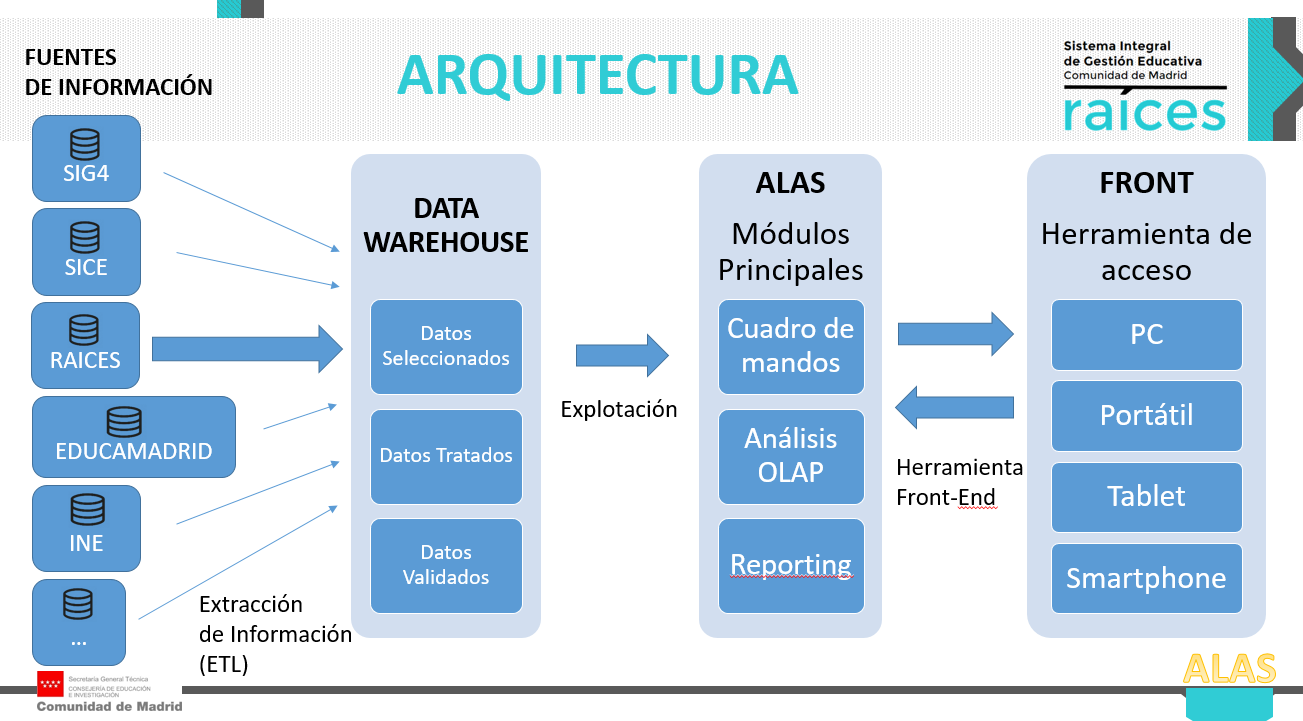
\includegraphics[width=0.8\textwidth]{recursos/arquitecturaDWH2}
	\label{fig:arquitecturaDWH2}
\end{figure*}
\FloatBarrier

%En la figura \ref{fig:arquitecturaDWH2} se muestra cuales son las fuentes de información, como se crea el ``DataWareHouse'' (que para entenderse son simplemente bases de datos con una estructura especial) y los módulos principales que se encargaran de seleccionar la información de una determinada forma para que posteriormente el usuario pueda visualizarla.
En primer lugar se tiene un gran numero de bases de datos de la CEI. A partir de los datos solicitados para realizar la explotación, se tiene que realizar la búsqueda en las tablas de estas bases de datos.

En segundo lugar, se crea un almacén de datos (Datawarehouse -DWH-), que son tablas dispuestas de una determinada forma o diseño (en este caso forma de estrella), donde se encuentran las tablas de hechos y las tablas de dimensiones. Las tablas de hechos son el corazón de un esquema en estrella, almacenan campos claves que se unen a las tablas de dimensiones, ademas incluyen métricas del negocio, contienen millones de registros. Las tablas de dimensiones son las que ofrecen mas información sobre características de las tablas de hechos, normalmente contienen pocos registros.
\begin{figure*}[h]
	\centering
	\caption{Esquema en estrella. Recuperado de http://carlospesquera.com}
	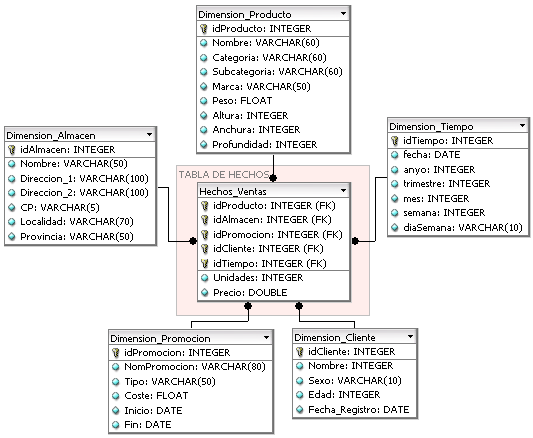
\includegraphics[width=0.8\textwidth]{recursos/Esquema_en_estrella}
	\label{fig:esquemaestrella}
\end{figure*}
\FloatBarrier

Cada tipo de diseño (en estrella o en copo de nieve), que permite realizar consultas multidimensionales, debe seleccionarse según las necesidades de los datos. Esta estructura en la base de datos es la clave para realizar los esquemas de Mondrian OLAP, conocidos como cubos de Mondrian. \cite{MONDRIAN}

\begin{figure*}[h]
	\centering
	\caption{Cubo de Mondrian. Recuperado de: https://www.businessintelligence.info}
	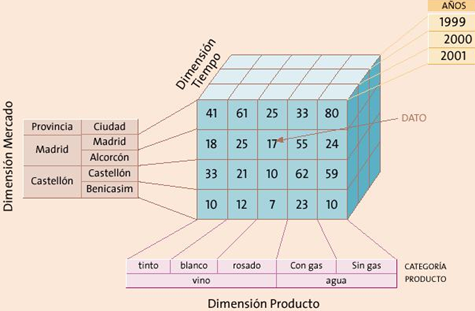
\includegraphics[width=0.8\textwidth]{recursos/modelo-dimensional-cubo}
	\label{fig:modelo-dimensional-cubo}
\end{figure*}
\FloatBarrier

Estos esquemas (que son archivos .XML) lo que hacen es ``traducir'' el diseño unidimensional de las tablas relacionales a un diseño multidimensional de forma que puedan ser entendidos por los servidores de Business Intelligence (BI). 

Para crear el esquema de Mondrian, primero se tiene que decidir cuales son las tablas de hechos y las tablas de dimensiones. Un ejemplo concreto sobre un diseño realizado en la CEI ha sido una tabla de hechos que contiene el identificador de centros, el numero de alumnos, el número de grupos, el nivel escolar, la naturaleza del centro (publico, privado o concertado), etc. La tabla de dimensiones contiene los propios valores de la tabla anterior, por ejemplo, para la columna naturaleza del centro de la tabla de hechos, existe una dimensión que contenga los valores público, privado o concertado.

Una vez que se tiene el diseño de tablas creado, ya se puede realizar la fase de extracción, transformación y carga (ETL); con la que se extraen los datos de la fuente de información, se producen las transformaciones oportunas y posteriormente dichos datos se almacenan en las tablas de hechos o dimensiones. A través de esta fase es donde se limpia los datos, eliminando las filas que no contengan todos los campos o rellenando los campos con algún valor en caso que fuera necesario.

Una vez que se tienen los datos limpios y cargados en las tablas de hechos y dimensiones, se tiene que subir el esquema al servidor y establecer una conexión con la base de datos, a partir de aquí, el trabajo es del motor OLAP del servidor, quien se encarga de traducir las opciones introducidas por el usuario en los cuadros de mandos a complejas consultas en la base de datos. 

En resumen, y a partir de los datos almacenados en el ``Datawarehouse''(DWH), la investigación que se lleva a cabo en este TFM se centra en analizar dichos datos. Pudiéndose recurrir a las fuentes de información originales para obtener nuevos datos en caso necesario. 

\section{Diseño de la minería de datos}
Una vez que se tiene claro la arquitectura principal del sistema, se establece el camino a seguir a la hora de realizar la investigación. Para ello, se utiliza la metodologia CRISP-DM. \citeA{IBMCRISP2012}

La metodología CRISP-DM tiene como objetivo orientar los proyectos de minería de datos. 
\begin{itemize}
	\item Como metodología: incluye descripciones de las fases normales de un proyecto, las tareas necesarias en cada una de las fases y una explicación de las relaciones entre las tareas.
	\item Como modelo de proceso: ofrece un resumen del ciclo vital de la minería de datos.
\end{itemize}

La metodología CRISP-DM establece un proceso genérico para satisfacer los objetivos deseados y contemplar la realización de la vigilancia e inteligencia. Este proceso se divide en distintas etapas básicas. 

\begin{figure*}[h]
\centering
\caption{Fases del ciclo de vida de CRISP-DM. Recuperado de \protect\citeA{IBMCRISP2012}.}
 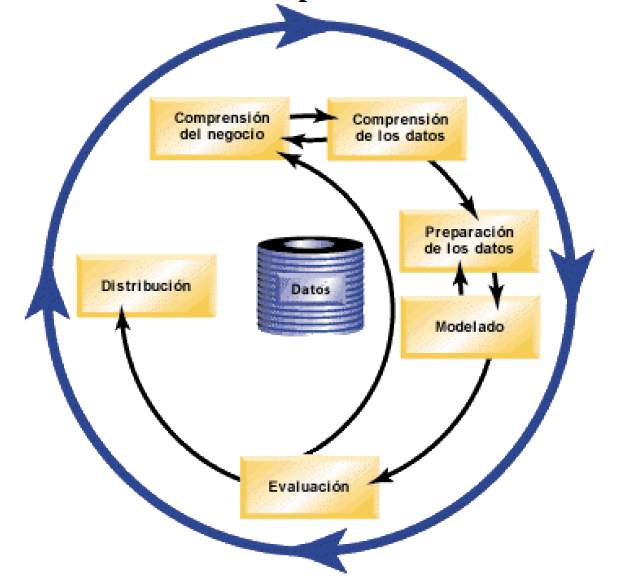
\includegraphics[width=0.6\textwidth]{recursos/CRISPCicloIBM}
\label{fig:CicloCrispDM}
\end{figure*}
\FloatBarrier
El ciclo de vida de CRISP-DM está compuesto de seis fases. La secuencia de estas no es estricta, es más, la mayoría de proyectos avanzan y retroceden entre fases si es necesario. En la figura \ref{fig:CicloCrispDM} se puede observar cada fase:

\begin{enumerate}
	\item \textbf{Comprensión del negocio.} Debe comprenderse los objetivos del negocio. Se debe realizar una descripción del problema. Por ultimo debe hacerse un plan de proyecto para alcanzar los objetivos deseados.
	\item \textbf{Comprensión de los datos.} Debe identificarse las fuentes de los datos y obtener aquellos datos relevantes para la consecución de los objetivos.
	\item \textbf{Preparación de los datos.} Conlleva el pre-procesado, la limpieza y la transformación de los datos relevantes con el objetivo de usar algoritmos de minería de datos.
	\item \textbf{Modelado.} Se debe desplegar un gran número de modelos y quedarse con aquellos que devuelvan valores óptimos para los datos utilizados.
	\item \textbf{Evaluación.} Debe evaluarse y probarse los modelos. Deben compararse entre sí y comprobar que son útiles para los datos expuestos.
	\item \textbf{Distribución.} Se realizan actividades usando los modelos seleccionados en el proceso de la toma de decisión.
\end{enumerate}

En los próximos puntos se va a describir las actividades que se realizan en cada una de estas fases.

\subsection{Comprensión del negocio}
La primera tarea a realizar en el ciclo de CRISP-DM es obtener la máxima información posible de los objetivos de esta investigación. Desde la CEI se ha comunicado la información disponible y las necesidades actuales.

Una de las necesidades de la CEI es obtener la máxima información sobre la situación actual de la educación en la comunidad de Madrid. La CEI posee una gran cantidad de datos de alumnos y centros a lo largo del tiempo. 

Por tanto, para sacar el mayor beneficio de los datos, se ha planteado el uso de herramientas y técnicas que posibiliten obtener información no solo del momento actual, sino también de la evolución a lo largo de los últimos años.

Una de las actividades que se han realizado es obtener el número de grupos y alumnos por centro, año, DAT, nivel educativo, etc.

Otra de las actividades que se realizan es obtener gráficos sobre la evolución de alumnos con necesidades especiales, alumnos de minorías étnicas e incluso porcentaje y nacionalidad de alumnos extranjeros.

\subsection{Comprensión de los datos}
Esta fase implica estudiar detalladamente los datos disponibles. Es esencial para evitar problemas inesperados durante la fase siguiente.

Para realizar esta fase, debemos tener en cuenta dos consideraciones relacionadas. La primera consideración es la identificación de necesidades de información y la segunda es la identificación de fuentes internas y externas.

\subsubsection{Identificación de necesidades de información}

Para realizar la identificación de las necesidades de información se va a partir de varios factores como son:
\begin{itemize}
	\item las demandas esperadas o manifestadas por (en este caso) una unidad de la consejería de educación.
	\item el análisis, la evolución de productos, procesos, materiales y tecnologías en el ámbito de la minería de datos educativa.
\end{itemize}

\subsubsection{Identificación de fuentes internas y externas de información}

Teniendo en cuenta las principales necesidades de información, se debe identificar las fuentes de información y recursos disponibles ya sean internos o externos a la organización. En este caso, utilizan las siguientes fuentes:
\begin{itemize}
	\item Fundamentalmente se utilizan documentos y recursos internos de la organización como: repositorios documentales, carpetas locales, bases de datos, etc.
	\item Personas con conocimientos o experiencias relacionadas con la necesidad de información. En este aspecto se realizan distintas reuniones con las personas encargadas de esta unidad de la consejería de educación. Para ello se realizarán reuniones con estos responsables. A partir de estas reuniones se obtendrán las fuentes de información.
	%\item Fuentes documentales a las que tiene acceso a la organización, ya sea en soporte físico (revistas, catálogos, etc.) como en soporte electrónico. Además, se utilizarán recursos de información en Internet (portales, noticias, redes sociales, foros, etc.). 
	\item Documentación técnica como reglamentaciones, especificaciones, propiedad industrial e intelectual o normas.
	\item Resultados de análisis existentes sobre las tendencias de futuro preferentemente en el ámbito educativo.
\end{itemize}

%\subsubsection{Búsqueda y tratamiento de la información}

La información fundamentalmente se encuentra en bases de datos internas, no obstante, se va a acceder a bases de datos externas en caso de necesidad para cumplimentar la información. 

En este aspecto, se debe recurrir a la ayuda de personas con conocimientos sobre el estado de las bases de datos. Como cualquier organización, la consejería de educación maneja grandes volúmenes de datos, por tanto, se debe tener conocimiento sobre donde se puede encontrar la información que satisfaga con las necesidades. 

El desconocimiento del estado de las bases de datos conlleva la inversión de una gran cantidad de tiempo en la búsqueda de los datos relevantes. 

De esta fase se espera localizar todos los datos que posteriormente se prepararan y se utilizaran en el modelado.

\subsection{Preparación de los datos}
Una vez que se tienen claros los datos que se utilizan, se procede a realizar la preparación para poder utilizarlos en la fase de modelado.

Algunas de las actividades que se realizan en esta fase son: la fusión de conjuntos y/o registros de datos, la selección de una muestra de un subconjunto, la agregación de registros, por contra la derivación de nuevos atributos a partir de anteriores, la eliminación o sustitución de valores en blanco o ausentes y por último la división de datos de prueba y entrenamiento.

Además, también se va a estudiar la existencia de datos perdidos y errores en estos.

Para realizar este tratamiento de datos se utilizará la técnica de ETL (extracción, transformación y carga) que consiste básicamente en obtener los datos de la fuente de origen (bases de datos, ficheros Excel, ficheros JSON, etc.), seleccionar aquellos datos que convengan al estudio, transformarlos según las necesidades que se tenga y depurarlos (evitando así datos erróneos). \cite{prakash2017etl} \cite{matos2006metodologia},\cite{gour2010improve}.
Para realizar este tratamiento, se ha va a utilizar Pentaho BI, que es un conjunto de programas libres para realizar entre otras muchas actividades, las técnicas de ETL. Concretamente, se ha utilizado la herramienta Spoon para desarrollar esta técnica. 
Una vez que se tienen los datos limpios y estructurados, se pueden realizar dos operaciones:

\begin{enumerate}
	\item  En primer lugar, se pueden almacenar dichos datos en una base de datos y seguir utilizando Pentaho BI para poder crear cuadros de mandos e informes o análisis OLAP. 
	
	\item  En segundo lugar, se puede almacenar la información en un texto plano para poder trabajar con herramientas de análisis descriptivo y predictivo. Estos análisis se realizan a través del entorno y lenguaje de programación R, que es una referencia en el ámbito de la estadística.
\end{enumerate}

\subsubsection{Análisis Exploratorio}

%El análisis predictivo (también conocido como estadísticas predictivas) se encarga de resumir los datos en bruto para que puedan ser interpretados. Estos análisis son útiles ya que permiten aprender sobre comportamientos o patrones pasados e entender cómo pueden influir en los resultados futuros. En este tipo de análisis se van a utilizar tanto métodos gráficos como medidas resumen.

La primera actividad en un análisis exploratorio es estudiar el tipo de datos de cada variable a investigar, se debe clasificar las variables según sean categóricas (dicotómicas o polinómicas) o numéricas (discretos o continuos). El tipo de datos permite decidir qué tipo de análisis estadístico utilizar.
Una vez que se tienen claro el tipo de datos utilizados, se utilizan los principales estadísticos como la media, la mediana, las desviaciones típicas, etc.
Posteriormente se va a utilizar la matriz de varianzas y covarianzas, que indicaran la variabilidad de los datos y la información sobre las posibles relaciones lineales entre las variables. 

Por otro lado, se va a estudiar la correlación de las variables mediante la matriz de correlación. Esta matriz contendrá los coeficientes de correlación.\cite{JMMarin}. La matriz de correlación, se utilizará fundamentalmente por pares entre las variables y la variable a predecir.

También se va a estudiar la matriz de correlaciones parciales, que estudia la correlación entre pares de variables eliminando el efecto de las restantes.\cite{JMMarin}

Los datos categóricos se representan en tablas de frecuencias, gráficos de barras y gráficos de sectores. Los datos numéricos se representan mediante histogramas, boxplot y diagramas QQ-Plot o Grafico Cuantil-Cuantil. \cite{Orellana2001}

Mediante el boxplot se puede observar aspectos como la posición, dispersión, asimetría, longitud de colas y los datos anómalos (outliers). 
El QQ-plot se va a utilizar para evaluar la cercanía de los datos a una distribución. \cite{Orellana2001}

%(https://www.sergas.es/gal/documentacionTecnica/docs/SaudePublica/Apli/Epidat4/Ayuda/Ayuda_Epidat_4_Analisis_descriptivo_Octubre2014.pdf)
Por otro lado, se va a complementar el análisis descriptivo mediante el aprendizaje no supervisado, donde también se extraerán otras características de los datos.

%En este apartado, se va a presentar la forma en la que se va a realizar la investigación. En primer lugar, se va a realizar un proceso ETL, posteriormente se va a realizar un análisis descriptivo mediante sus técnicas que se explicaran posteriormente, además se va a incluir técnicas de aprendizaje no supervisada en este análisis.
%Una vez que se ha realizado el análisis descriptivo, se va a realizar un análisis predictivo. En este análisis se va a utilizar técnicas de aprendizaje supervisadas.


\subsection{Modelado}
Una vez terminado el análisis descriptivo, se va a realizar un análisis predictivo. Se debe tener en cuenta, que, dentro de la ciencia de datos, existen técnicas de aprendizaje automáticas, cuyo objetivo es la construcción de un sistema que sea capaz de aprender a resolver problemas sin la intervención de un humano. \cite{MARIN2018}.

Las técnicas de aprendizaje tienen como resultado un modelo para resolver una tarea dada. Los modelos son una representación de la realidad basado en un intento descriptivo de relacionar un conjunto de variables con otro.

Los modelos predictivos son de dos tipos: regresión, que son capaces de predecir una respuesta cuantificable; y de clasificación, que son capaces de predecir respuesta categóricas.

\subsubsection{Aprendizaje automático}
%https://www.fisterra.com/mbe/investiga/10descriptiva/10descriptiva.asp#top
%http://www.uco.es/zootecniaygestion/img/pictorex/27_12_49_7.pdf
%https://machinelearningmastery.com/descriptive-statistics-examples-with-r/
%http://cms.dm.uba.ar/academico/materias/verano2015/estadisticaQ/descriptiva.pdf

El \textbf{aprendizaje supervisado} consiste en la búsqueda de patrones en datos históricos relacionando todas las variables con una especial (conocida como variable objetivo). Los algoritmos que se utilizan en el aprendizaje supervisado se encarga de buscar patrones en los datos. A este proceso se conoce como entrenamiento de los datos. Una vez que se tienen los patrones, se aplican a los datos de prueba. Los datos de entrenamiento suelen ser una selección aleatoria y única de los datos históricos de un 70\% del total. Los datos de prueba son el restante 30\%. \cite{Manguart2017}.
Algunos de los algoritmos que se utilizan son:
\begin{enumerate}
	\item \textbf{Arboles de decisión}
	
	Se basa en el descubrimiento de patrones a partir de ejemplos. Un árbol de decisión está formado por un conjunto de nodos (de decisión) y de hojas (nodos-respuesta).
	
	Los nodos están asociados a los atributos y tiene varias ramas que salen de él (dependiendo de los valores que tomen la variable asociada). Estos nodos pueden asemejarse a preguntas que, dependiendo de la respuesta que conlleve, se tomara un flujo en las ramas salientes.
	
	Los nodos respuesta están asociados a la clasificación que se desea proporcionar, devolviendo así la decisión del árbol con respecto al ejemplo de entrada utilizado.
	
	\begin{figure*}[htb]
		\centering
		\caption{Funcionamiento Árboles Decisión. Recuperado de \protect\citeA{sayad2019}}
		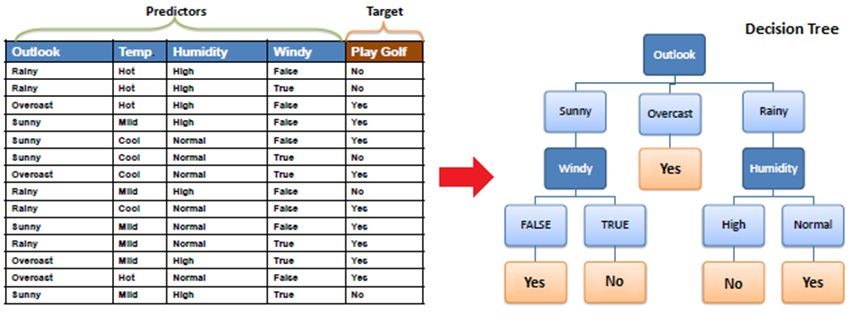
\includegraphics[width=0.8\textwidth]{recursos/arbol_decision_img1}
		\label{fig:fun_arb_dec}
	\end{figure*}
	\FloatBarrier

	
	\begin{comment}
	\item \textbf{Clasificación de Naïve Bayes}
	
	Es un algoritmo que se basa en la técnica de clasificación utilizando el teorema de Bayes.
	
	El algoritmo es capaz de agrupar un registro mediante las características de este. Para ello aplica probabilidades condicionales de las características para determinar a qué categoría pertenece. 
	
	Por ejemplo, una fruta puede considerarse una manzana si es de color rojo, redonda y tiene un determinado peso.
	
	\begin{figure*}[htb]
		\centering
		\caption{Teorema de Bayes. Recuperado de \protect\cite{uCincinnati2018}}
		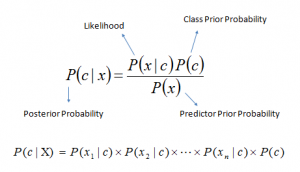
\includegraphics[width=0.6\textwidth]{recursos/BayesFormula}
		\label{fig:BayesFormula}
	\end{figure*}
	\FloatBarrier
	\end{comment}
	
	\item \textbf{Regresión Logística}
	
	Es un algoritmo de regresión que se utiliza para predecir el resultado de una variable categórica en función de las variables independientes o predictores. Para predecir el resultado, se establecen pesos en función de la puntuación dada a cada variable independiente.
	
	\item \textbf{Redes Neuronales}
	%https://www.tuinteligenciaartificial.es/las-redes-neuronales-en-la-inteligencia-artificial-explicacion-clara-y-sencilla/
	
	Las redes neuronales son un algoritmo de inteligencia artificial que se inspira en los mecanismos presentes en la naturaleza. Las neuronas envían señales eléctricas de manera fuerte o débil a otras neuronas. La combinación de todas las conexiones entre neuronas es lo que genera el conocimiento. Estas señales se envían cuando existe unos estímulos (inputs) externos a través de los sentidos. A lo largo de la vida, las neuronas aprenden que deben hacer a partir de dichos estímulos y, por lo tanto, los seres vivos aprenden a actuar ante distintas señales y situaciones. El funcionamiento de las redes neuronales en la inteligencia artificial es similar.
	
	\begin{figure*}[htb]
		\centering
		\caption{Red Neuronal. Recuperado de \protect\citeA{yepes2017}}
		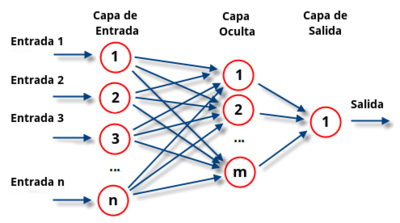
\includegraphics[width=0.6\textwidth]{recursos/RedNeuronalArtificial}
		\label {fig:RedNeuronal}
	\end{figure*}
	\FloatBarrier
	
	Como se puede observar en la figura \ref{fig:RedNeuronal}, la primera fila (con neuronas de color rojo), se conocen como nodos de entrada y son aquellos que se encargan de recoger la información. Los nodos en la gama azul son los que se conocen como nodos de salida. Los nodos situados en el medio son aquellos que se encargan de hacer el aprendizaje, y se conocen como nodos ocultos.
	
	En primer lugar, se obtiene la información a partir de los nodos de entrada, una vez que se tiene la información, se envía a las capas ocultas, que se activan o no dependiendo del aprendizaje previo. Los nodos ocultos se activan dependiendo de una serie del resultado de unas operaciones matemáticas. Si los nodos se activan, entonces enviaran la información a la siguiente capa.
	
	\item \textbf{Bosques aleatorios}
	
	Los bosques aleatorios son un método que se encarga de combinar los resultados de árboles de decisión independientes.
	
	Algunas características son:
	\begin{itemize}
		\item Gran precisión.
		\item Eficiente para grandes bases de datos.
		\item Aporta estimaciones sobre la importancia de las variables en la clasificación.
		\item Tiene un método eficaz para la estimación de los datos faltantes y mantiene la precisión cuando falta una gran parte de los datos.
	\end{itemize}
	%https://quantdare.com/random-forest-vs-simple-tree/
	%http://randomforest2013.blogspot.com/2013/05/randomforest-definicion-random-forests.html
	%https://bookdown.org/content/2031/ensambladores-random-forest-parte-i.html
	
	\item \textbf{Maquinas de Vectores Soporte (SVM)}
	Constituyen un método basado en el aprendizaje para la resolución de problemas de clasificación y regresión. Para ello, recibe unas entradas y obtienen unas salidas. Busca por tanto la curva/linea que modele la tendencia de los datos.
	
	Por ejemplo, si tenemos un anuncio en una pagina web y queremos analizar la edad y la hora del día del usuario que hace clic o no en dicho anuncio, con SVN se obtiene la "superficie optima" que delimitara el comportamiento (clic-noclic) de un determinado usuario. \cite{JANA2016}
	
		\begin{figure*}[htb]
		\centering
		\caption{Ejemplo SVM. Recuperado de \protect\citeA{JANA2016}}
		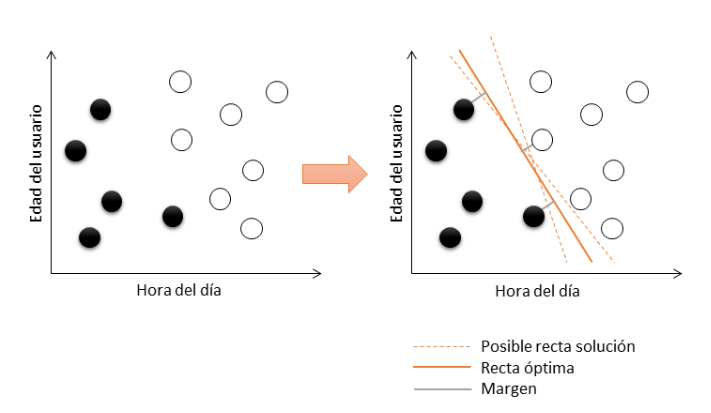
\includegraphics[width=0.6\textwidth]{recursos/SVM}
		\label {fig:SVM}
	\end{figure*}
	\FloatBarrier
	
	\item \textbf{K-Vecinos-cercanos}
	
	K-vecinos-cercanos (conocido también como K-NN) es un algoritmo de aprendizaje supervisado en el que, a partir de unos datos iniciales, es capaz de clasificar todas las nuevas instancias.
	
	La idea es que el algoritmo clasifica cada dato nuevo en el grupo que corresponda, según cual sea el grupo vecino (de los k grupos) más próximo. Por tanto, calcula la distancia del elemento nuevo a cada uno de los existentes e indica a que grupo debe permanecer este nuevo elemento según la menor distancia.
	
	\begin{figure*}[htb]
		\centering
		\caption{KNN. Recuperado de \protect\citeA{klein2018}}
		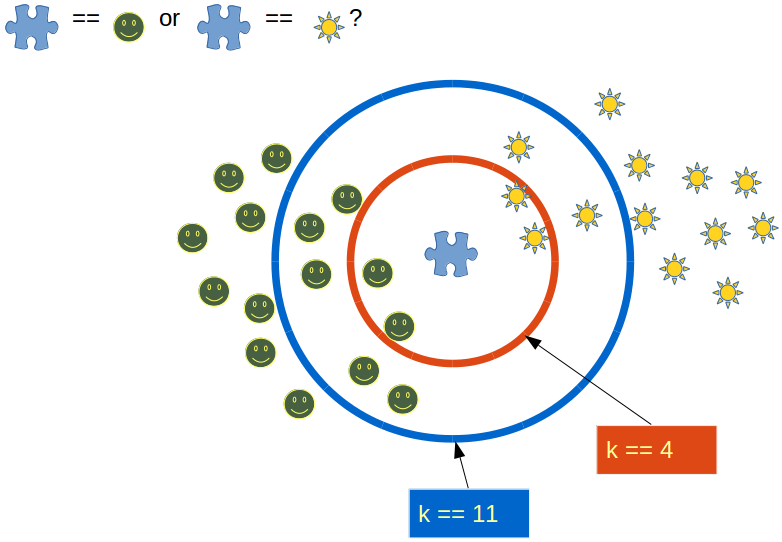
\includegraphics[width=0.6\textwidth]{recursos/k_NN}
		\label {fig:KNN}
	\end{figure*}
	\FloatBarrier
	
	
\end{enumerate}

\subsubsection{Criterio de selección}

Una vez que se han seleccionado las variables y los algoritmos a estudiar, es hora de realizar el propio modelado. Al realizar el modelado, debemos tener en cuenta que variables son mejores para este modelado. Es posible que existan variables que únicamente empeoren los resultados del modelado, por lo tanto, se deberán desestimar. Para ello se va a utilizar el criterio de Akaike (AIC). 

Este criterio indica el ajuste que tienen los datos experimentales con el modelo utilizado. Obviamente, el criterio de AIC solo tiene sentido cuando se realizan comparaciones con otros modelos (utilizando el mismo conjunto de datos). \cite{martinez2009criterio}

Cuanto menor sea el valor de este criterio, mejor se ajustan los datos al modelo. Por tanto, se deberá seleccionar el modelo que menor AIC tenga. \cite{martinez2009criterio}

\subsection{Evaluación}
En esta fase de la metodologia, se diferencian varias partes. La primera parte es la evaluación del propio modelo respecto a otros, por lo que se utilizaran las métricas de precisión. La segunda parte va a ser la evaluación de la propia Unidad de Secundaria la que evalúe los resultados de predicción obtenidos para un determinado curso con los existentes en la realidad para dicho curso.

\textbf{Métricas de precisión}
El error absoluto medio (MAE) y el error cuadrático medio (RMSE) son dos de ls métricas mas comunes utilizadas para medir la precisión de las variables continuas en los modelos de regresión.

\textbf{Error absoluto medio (MAE):} mide la magnitud promedio de los errores en un conjunto de predicciones, sin considerar su dirección. Es el promedio sobre la muestra de prueba de la diferencia absoluta entre la predicción y la observación real.
\begin{figure*}[h]
	\centering
	\caption{Fórmula de MAE. Recuperado de https://medium.com/human-in-a-machine-world/mae-and-rmse-which-metric-is-better-e60ac3bde13d}
	\includegraphics[width=0.4\textwidth]{recursos/mae}
	\label{fig:MAE}
\end{figure*}
\FloatBarrier
Error cuadrático medio (RMSE): es una regla de puntuación cuadrática que mide la magnitud promedio del error. Es la raíz cuadrada del promedio de las diferencias cuadradas entre la predicción y la observación real.
\begin{figure*}[h]
	\centering
	\caption{Fórmula de RMSE. Recuperado de https://medium.com/human-in-a-machine-world/mae-and-rmse-which-metric-is-better-e60ac3bde13d}
	\includegraphics[width=0.4\textwidth]{recursos/rmse}
	\label{fig:MAE}
\end{figure*}
\FloatBarrier

Se debe destacar que cuanto menos sea el error, más se acercan los datos predichos a la realidad.

\begin{comment}
Las métricas que se va a utilizar para obtener la precisión de los modelos son aquellas descritas en el artículo de  \citeA{COSTA2017247}, \citeA{Helal2018} y \citeA{ASHRAF20181021}. Estas métricas son frecuentes en ámbitos como la obtención de información, aprendizaje automático y otros dominios como la clasificación binaria. Dichas métricas son las siguientes:

\begin{itemize}
	\item FMeasure: es la media armónica de la precisión y recuperación de un clasificador; es decir, FMeasure = 2 * Precision * Recall / (Precision + Recall).
	\item Precision: es la fracción de verdaderos positivos entre todos los ejemplos clasificados como positivos. P= TP/(FP+TP).
	\item Recall: es la fracción de verdaderos positivos clasificados correctamente. R = TP/(FN+TP).
	\item AUC: el área bajo la característica de operación del receptor. La curva (ROC) indica la probabilidad de que un clasificador clasifique un positivo seleccionado aleatoriamente sobre un negativo. Un AUC con valor de 1 indica un perfecto clasificador, mientras que 0.5 implica que el clasificador lo hace de forma aleatoria.
\end{itemize}

Donde:
\begin{itemize}
	\item TP - Verdadero Positivo: es el número de instancias positivas clasificadas correctamente como positivas. 
	\item FP - Falso Negativo: es el número de instancias positivas clasificadas incorrectamente como negativas.
	\item FP - Falso Positivo: es el número de instancias negativas clasificadas incorrectamente como positivas.
	\item TN - Verdadero Negativo: es el número de instancias negativas clasificadas correctamente como negativas.
\end{itemize}

Estas métricas se muestran utilizando un gráfico conocido como matriz de confusión.

\end{comment}
\subsection{Distribución}
La fase de distribución considera la planificación y control de la distribución de los resultados. Debe tener en cuenta la realización de un informe final.

Respecto a la fase de distribución, se utilizan los modelos generados para predecir datos de otros cursos. Concretamente se utiliza el modelo que mayor precisión obtiene con los datos aportados.

Concretamente, los datos utilizados en la predicción son aquellos del curso 2016/2017. A partir de estos datos, se obtienen varios modelos. Una vez que se ha seleccionado el mejor modelo, ya se puede utilizar otro conjunto de datos. En este caso, el conjunto de datos a utilizar es el del curso 2017/2018.

Esta fase, por tanto, aplicada a un entorno empresarial, debería indicar que modelos deben integrarse en el sistema. En este entorno académico, simplemente se debe indicar el mejor modelo y una comparativa de todos los modelos utilizados.




 %esta no podrá salir de la CEI. Aunque se trate de datos anonimizados y agregados, se trata de datos de carácter sensible y no pueden ser distribuidos. Por tanto, dichos datos se almacenan en un gestor de bases de datos MySQL. Este gestor se encontrará en un servidor de la Consejería de Educación e Investigación. Solo se va a poder acceder a dicho servidor desde la propia sede. Es posible que los datos también se almacenen en archivos de texto plano.

\section{Herramientas utilizadas}
\subsection{Suite de Pentaho BI}
Para el desarrollo del proyecto, se tiene en cuenta la posibilidad de utilizar la herramienta de Pentaho Business Analytics, que es una suite de herramientas para la explotación de datos. Esta suite posee las herramientas que se usan y son las siguientes: Spoon, Pentaho SchemaWorkbench y Pentaho Metadata Editor.

\subsection{Lenguaje R y RStudio}
En esta línea de investigación se va a utilizar R como lenguaje de programación y RStudio como entorno de desarrollo para R.

Como ya se ha comentado, R es un lenguaje de programación para el análisis estadístico. Al estar orientado a la estadística, proporciona un gran número de bibliotecas y herramientas. Destaca también por la generación de gráficos estadísticos de gran calidad. Posee muchos paquetes dedicados a la graficación. Además, es una herramienta que facilita el cálculo numérico y el uso en la minería de datos. \cite{emanuel2014}

Su potencia reside fundamentalmente en que es un software gratuito y de código abierto. Como ya se ha comentado, posee un gran número de herramientas que pueden ampliarse mediante paquetes, librerías o definiendo funciones propias.

Por otro lado, RStudio es el entorno de desarrollo para R. Es también software libre y tiene la ventaja que se puede ejecutar sobre distintas plataformas (Windows, Mac y Linux).

\subsubsection{El Paquete \textit{Caret}}

El paquete \textbf{caret} es un conjunto de funciones que intenta agilizar el proceso de creación de modelos predictivos. El paquete contiene herramientas para: división de datos, pre-procesamiento, selección de características, ajuste del modelo mediante re-muestreo, estimación de importancia variable así como otras funcionalidades. \cite{CARET2019}



